%%%%%%%%%%%%%%%%%%%%%%%%%%%%%%%%%%%%%%%%%%%%%%%
%%%     Declarations (skip to Begin Document, line 101, for parts you fill in)
%%%%%%%%%%%%%%%%%%%%%%%%%%%%%%%%%%%%%%%%%%%%%%%

\documentclass[10pt]{article}

\usepackage{geometry}  % Lots of layout options.  See http://en.wikibooks.org/wiki/LaTeX/Page_Layout
\geometry{letterpaper}  % ... or a4paper or a5paper or ... 
\usepackage{fullpage}  % somewhat standardized smaller margins (around an inch)
\usepackage{setspace}  % control line spacing in latex documents
\usepackage[parfill]{parskip}  % Activate to begin paragraphs with an empty line rather than an indent

\usepackage{url}

\usepackage{amsmath,amssymb}  % latex math
\usepackage{empheq} % http://www.ctan.org/pkg/empheq
\usepackage{bm,upgreek}  % allows you to write bold greek letters (upper & lower case)

% allows strikethroughs in math via \cancel{math text goes here}
\usepackage{cancel}

% provides adjustwidth environment to temporarily change margins
% \begin{adjustwidth}{left change length}{\right change length}
\usepackage{changepage}

% for typsetting algorithm pseudocode see http://en.wikibooks.org/wiki/LaTeX/Algorithms_and_Pseudocode
\usepackage{algorithmic,algorithm}  

\usepackage{graphicx}  % inclusion of graphics; see: http://en.wikibooks.org/wiki/LaTeX/Importing_Graphics
% allow easy inclusion of .tif, .png graphics
\DeclareGraphicsRule{.tif}{png}{.png}{`convert #1 `dirname #1`/`basename #1 .tif`.png}

\usepackage{subfigure}  % allows subfigures in figure
%\usepackage{caption}
%\usepackage{subcaption}

\usepackage{xspace}
\newcommand{\latex}{\LaTeX\xspace}

\usepackage{color}  % http://en.wikibooks.org/wiki/LaTeX/Colors

\long\def\ans#1{{\color{blue}{\em #1}}}
\long\def\ansnem#1{{\color{blue}#1}}
\long\def\boldred#1{{\color{red}{\bf #1}}}
\long\def\boldred#1{\textcolor{red}{\bf #1}}
\long\def\boldblue#1{\textcolor{blue}{\bf #1}}
\long\def\todo#1{\textcolor{red}{\bf TODO: #1}}

% misc math defs
\newcommand{\norm}[1]{\left\lVert#1\right\rVert}

% Useful package for syntax highlighting of specific code (such as python) -- see below
\usepackage{listings}  % http://en.wikibooks.org/wiki/LaTeX/Packages/Listings
\usepackage{textcomp}

%%% The following lines set up using the listings package
\renewcommand{\lstlistlistingname}{Code Listings}
\renewcommand{\lstlistingname}{Code Listing}

%%% Specific for python listings
\definecolor{gray}{gray}{0.5}
\definecolor{green}{rgb}{0,0.5,0}

\lstnewenvironment{python}[1][]{
\lstset{
language=python,
basicstyle=\footnotesize,  % could also use this -- a little larger \ttfamily\small\setstretch{1},
stringstyle=\color{red},
showstringspaces=false,
alsoletter={1234567890},
otherkeywords={\ , \}, \{},
keywordstyle=\color{blue},
emph={access,and,break,class,continue,def,del,elif ,else,%
except,exec,finally,for,from,global,if,import,in,i s,%
lambda,not,or,pass,print,raise,return,try,while},
emphstyle=\color{black}\bfseries,
emph={[2]True, False, None, self},
emphstyle=[2]\color{green},
emph={[3]from, import, as},
emphstyle=[3]\color{blue},
upquote=true,
morecomment=[s]{"""}{"""},
commentstyle=\color{gray}\slshape,
emph={[4]1, 2, 3, 4, 5, 6, 7, 8, 9, 0},
emphstyle=[4]\color{blue},
literate=*{:}{{\textcolor{blue}:}}{1}%
{=}{{\textcolor{blue}=}}{1}%
{-}{{\textcolor{blue}-}}{1}%
{+}{{\textcolor{blue}+}}{1}%
{*}{{\textcolor{blue}*}}{1}%
{!}{{\textcolor{blue}!}}{1}%
{(}{{\textcolor{blue}(}}{1}%
{)}{{\textcolor{blue})}}{1}%
{[}{{\textcolor{blue}[}}{1}%
{]}{{\textcolor{blue}]}}{1}%
{<}{{\textcolor{blue}<}}{1}%
{>}{{\textcolor{blue}>}}{1},%
%framexleftmargin=1mm, framextopmargin=1mm, frame=shadowbox, rulesepcolor=\color{blue},#1
framexleftmargin=1mm, framextopmargin=1mm, frame=single,#1
}}{}
%%% End python code listing definitions

\DeclareMathOperator{\diag}{diag}
\DeclareMathOperator{\cov}{cov}

%%%%%%%%%%%%%%%%%%%%%%%%%%%%%%%%%%%%%%%%%%%%%%%
%%%     Begin Document
%%%%%%%%%%%%%%%%%%%%%%%%%%%%%%%%%%%%%%%%%%%%%%%

\begin{document}

\begin{center}
    {\Large {\bf ISTA 421 / INFO 521 - Homework 1}} \\
    \boldred{Due: Friday, August 31, 5pm} \\
    24 points total (same for undergraduates and graduates) \\
    \vspace{1cm}
\end{center}

\begin{flushright}
STUDENT NAME  %% Fill in your name here

Undergraduate / Graduate %% select which you are!
\end{flushright}

\vspace{1cm}

{\Large {\bf Instructions}}

On this (and other ``regular'' -- i.e., non-midterm/final assignments) you may {\em discuss} problems with others in the class, BUT your code and written solutions \boldred{MUST BE YOUR OWN}.  Do not copy code or written solutions by others.  Copying is cheating.

{\bf If you work with others, you must include in your submission a list of people you talked with.  If you reference other material (fine to do!), you must cite those resources.}

Include in your final submission the pdf of written answers along with separate files for any python scripts that you write in support of answering the questions. 
You are required to create either a .zip or tarball (.tar.gz / .tgz) archive of all of the files for your submission and submit the archive to the D2L dropbox by the date/time deadline above.
Refer to the course submission instructions at: \\
\url{http://w3.sista.arizona.edu/~clayton/courses/ml/submissions.html}

In future problem sets, there will be additional or different problems that graduate students must complete, but in this case, everyone must do the same problems for the same points.

Mathematical content: This is a mathematical subject and there is a wide variance in backgrounds of students who take this course. For example, there may be problems in the assignments which seem more difficult than they really are simply because you are not (yet) used to the kind of problem. 

The purpose of this assignment is to learn (or remember) how to write short programs to explore mathematical ideas. It was written on the assumption that you will use Python for your assignments (recommended). If you wish do some of the tasks in a different language you may need to adjust the questions a little bit, but what goes into the PDF (e.g., plots, answers) should be the same. 

Most of the problems below have multiple parts.  In most cases, what is being asked for is clearly indicated by the explicit question(s) or request(s) (e.g., exercise 5 clearly asks you to show two different equations between scalar and vector notation hold).  Some exercises (e.g., exercise 6) have a flavor of a ``tutorial''.  For these problems, I add a (\$) for each part of the exercise that requires an explicit answer.  Each (\$) is worth an equal proportion of the total points for that exercise; e.g., exercise 6 is worth 5 points total and there are 10 (\$)s, so each is worth 0.5 points.

In the following, FCMA refers to the course text: Simon Rogers and Mark Girolami (2012), {\em A First Course in Machine Learning}, first edition.  (All questions from the book are reproduced here in full, so you do not need the book to proceed.)

For general notes on using latex to typeset math, see: {\tt http://en.wikibooks.org/wiki/LaTeX/Mathematics}

{\bf Always start assignments ASAP, do {\em NOT} wait until the last couple of days.}

\vspace{.5cm}

%%%%%%%%%%%%%%%%
%%%     Problems
%%%%%%%%%%%%%%%%

\newpage
\begin{enumerate}


%%%   Problem 1
\item \label{prob:1} [0 points]
If you haven't already, setup your programming environment!  Python is highly recommended:\\
\url{http://w3.sista.arizona.edu/~clayton/courses/ml/python_setup.html}

If python is new to you, work through the short python tutorial:\\
\url{http://w3.sista.arizona.edu/~clayton/courses/ml/tutorial.html}

See the Appendix at the end of these instructions for additional information about numpy, arrays and matrices.



%%%   Problem 2
\item \label{prob:2} [1 point]
{\bf Exercise 1.1} from FCMA p.35

\begin{figure}[htb]
\begin{center}
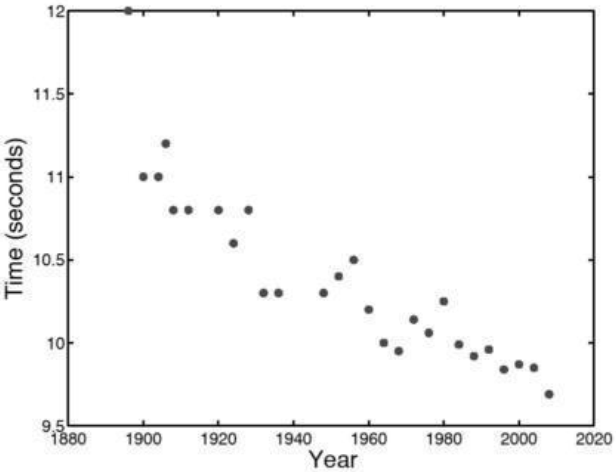
\includegraphics[width=6cm]{figures/figure1-1_p2}
\caption{Reproduction of figure 1.1, Olympic men's 100m data}
\end{center}
\end{figure}
By examining Figure 1.1 [from p. 2 of FCMA, reproduced here], estimate (by hand / in your head) the kind of values we should expect for $w_0$ (y-intercept) and $w_1$ (slope) as parameters of a line fit to the data (e.g., High? Low?  Positive?  Negative?).  (No computer or calculator calculation is needed here -- just estimate!)

{\bf Solution.} $<$Solution goes here$>$\\


\newpage
%%% Note for next three problems:
NOTE: The following three exercises (3, 4 and 5) review basic linear algebra concepts.
% \begin{enumerate}

\item[] Notation conventions:
\begin{itemize}
\item Script variables, such as $x_{n2}$ and $w_1$ represent scalar values
\item Lowercase bold-face variables, such as $\mathbf{x}_n$ and $\mathbf{w}$, represent vectors
\item Uppercase bold-face variables, such as $\mathbf{X}$, represent $n$ (rows) $\times ~m$ (columns) matrices
\item Note that because all indexes in the following are either a single digit integers (0, 1, ..., 9), or a single letter representing an integer index, e.g., $n$, I am representing multiple dimension indexes without a comma, as it is unambiguous; e.g., $x_{32}$ is the element scalar value of $\mathbf{X}$ at row 3, column 2.  When we have to refer to specific index values greater than 9, we'll use commas, such as $x_{32,3}$ is the scalar value in the 32nd row and 3rd column.
\item `$\top$' in expressions like $\mathbf{w}^\top$ indicates the {\em transpose} operator.
\item Unless stated otherwise, we will assume that all vectors {\em without} the transpose, $\top$, are {\em column} vectors, so $\mathbf{w}^\top$ is a {\em row vector}.
\item It is sometimes convenient to express an example vector as a bracketed list of elements (e.g., in a sentence): $[x_1, x_2, ..., x_n]$.  In general I am going to try to be careful about the orientation of vectors, so the previous example would be a {\em row} vector.  To make it a column vector, I'll add a transpose: $[x_1, x_2, ..., x_n]^\top$.
\end{itemize}



%%%   Problem 3
\item \label{prob:3} [2 points]
{\bf Exercise 1.3} from FCMA p.35

Show that:
\begin{eqnarray*}
\mathbf{w}^\top\mathbf{X}^\top\mathbf{X}\mathbf{w} = w_0^2 \left( \sum_{n=1}^N x_{n1}^2 \right) + 2w_0w_1 \left( \sum_{n=1}^N x_{n1}x_{n2} \right) + w_1^2 \left( \sum_{n=1}^N x_{n2}^2 \right),
\end{eqnarray*}
where
\begin{eqnarray*}
\mathbf{w} = 
    \begin{bmatrix}
    w_0 \\[0.3em]
    w_1
    \end{bmatrix}
    ,
\mathbf{X} = 
    \begin{bmatrix}
    x_{11} & x_{12} \\[0.3em]
    x_{21} & x_{22} \\[0.3em]
    x_{31} & x_{32} \\[0.3em]
    \vdots & \vdots \\[0.3em]
    x_{N1} & x_{N2}
    \end{bmatrix}
    .
\end{eqnarray*}
(Hint -- it's probably easiest to do the $\mathbf{X}^\top\mathbf{X}$ first!)

{\bf Solution.} $<$Solution goes here$>$\\


%%%   Problem 4
\item \label{prob:4} [1 point]
{\bf Exercise 1.4} from FCMA p.35

Using $\mathbf{w}$ and $\mathbf{X}$ as defined in the previous exercise, show that ${(\mathbf{X}\mathbf{w})}^\top = {\mathbf{w}}^\top{\mathbf{X}}^\top$ by multiplying out both sides.

{\bf Solution.} $<$Solution goes here$>$\\



%%%   Problem 5
\item \label{prob:5} [2 points]
{\bf Exercise 1.5} from FCMA p.35  % [1pt]

When multiplying a scalar by a vector (or matrix), we multiply each element of the vector (or matrix) by that scalar.  For $\mathbf{x}_n = {[ x_{n1}, x_{n2} ]}^\top$, $\mathbf{t} = {[ t_1,...,t_N ]}^\top$, $\mathbf{w} = {[ w_0, w_1 ]}^\top$, and
\begin{eqnarray*}
\mathbf{X} = 
    \begin{bmatrix}
    {\mathbf{x}_{1}}^\top \\[0.3em]
    {\mathbf{x}_{2}}^\top \\[0.3em]
    \vdots \\[0.3em]
    {\mathbf{x}_{N}}^\top
    \end{bmatrix}
\end{eqnarray*}
show that
\begin{eqnarray*}
\sum_{n} \mathbf{x}_n t_n = \mathbf{X}^\top\mathbf{t}
\end{eqnarray*}
and
\begin{eqnarray*}
\sum_{n} \mathbf{x}_n \mathbf{x}_n ^\top \mathbf{w} = \mathbf{X}^\top\mathbf{X} \mathbf{w}
\end{eqnarray*}

{\bf Solution.} $<$Solution goes here$>$\\


\newpage
%%%   Problem 6
\item \label{prob:6} [5 points]
Reading and Displaying Numpy Arrays:

Write a script, called `hw1.py', that uses the numpy function {\tt loadtxt} to load the contents of {\tt humu.txt} (available in the {\tt data/} subdirectory of the release) into a variable (\$).

{\em Hint: If {\tt loadtxt} is new to you, visit} \\
\url{http://docs.scipy.org/doc/numpy-1.13.0/reference/generated/numpy.loadtxt.html} {\em ; \\ in general python, numpy, scipy and matplotlib all have great online documentation!  Also, keep in mind that you will need to {\tt import numpy} at the top of your script in order to access numpy functions; I recommend avoiding using {\tt from numpy import *} as that pollutes your namespace and can lead to very hard to debug errors. }

The default output of {\tt loadtxt} is a numpy ndarray.  You can show this by getting the {\tt type} of the variable.  From the python terminal you could do this by entering {\tt type(var)}, or if you are executing your script and want to see the output, add a print statement: {\tt print(type(var))}.  In python 3.6, the output should be {\tt <class 'numpy.ndarray'>} .  Have your script print the type (\$).

You can get the total size of a numpy object using the {\tt size} field: {\tt var.size}.  {\tt size} holds the total number of elements in the array.  Google (or other search) ``numpy size'' to see the documentation about this field.  Have your script print the size of the loaded humu data (\$).

Knowing the (total) size is helpful, but in this case we are working with a 2-dimensional array, so it would be useful to get the array dimensions.  The numpy ndarray field {\tt shape} holds a tuple representing size of each dimension of the array.  Look at the documentation for numpy {\tt shape}.  Have your script print the shape of the loaded humu data (\$).

{\em Hint: To store both the width and height into variables in one go, try: {\tt h, w = var.shape}.  This is an example of ``unpacking'', and you can even do this with nested patterns: {\tt a, (b, c) = [1, [2, 3]]}.  You could alternately do: {\tt h = var.shape[0]} and {\tt w = var.shape[1]}.}

What is the range of values contained within the array?  Use the {\tt min} and {\tt max} functions to figure this out.  Have your script print the min and max values of the array (\$).

{\em Hint: take a look at the related {\tt amin} and {\tt amax} functions for full documentation.}

Use the {\tt min} and {\tt max} values to scale the values in your humu array so that they lie in the range $[0, 1]$ -- store this in a new array (\$).  Verify that the new, scaled array has the same dimensions as the original (print the shape!) but that the new values are in the range $[0, 1]$ (print the min and max of the new array!) (\$).

You will now use matplotlib to plot the original (not the scaled) image.  To do so, you need to do the following:
\begin{enumerate}
\item Add {\tt import matplotlib.pyplot as plt} to the top of your file.
\item Add {\tt plt.figure()} to create a new figure object
\item Use {\tt imshow} to display your original humu array.
\end{enumerate}
If you successfully do the above and run your script, it will likely open the figure very quickly and then close it right after (if it shows anything at all).  To get the figure to hang around, add: {\tt plt.show()}.  Note: the figure will stay open and python will not continue further script execution until after you close the figure.

Why does the plot look so strange?  Print the current colormap: {plt.cm.cmapname} -- this will print the default colormap name (which is likley `afmhot', matplotlib's version of Matlab's {\tt jet}, or `Vega20c\_r').  This is the default colormap that is useful for data visualization.  Try plotting your figure again, but this time, select the `gray' scale colormap by adding the following argument to {\tt imshow}: {\tt cmap='gray'} (\$).

{\em Note: specifying the colormap in imshow does not change the default colormap.}

{\em Tip: visit} \url{http://matplotlib.org/1.2.1/examples/pylab_examples/show_colormaps.html} {\em to see a list of available colormaps.  You can also create your own colormaps:}\\
\url{http://matplotlib.org/examples/pylab_examples/custom_cmap.html}\\
\url{http://stackoverflow.com/questions/16834861/create-own-colormap-using-matplotlib-and-plot-color-scale}

Now make a grayscale image that is the same size as the one we have been using, except create the values to be uniformly random (see the function {\tt numpy.random.random()}).  Does it look like what you expected?  Create a second such image.  Does it look much different? (\$)

Write the uniformly random array to a file called `random.txt' using the numpy {\tt savetxt} function.  Confirm (1) that you can read the result by opening the file in a text editor, and (2) that you can load it back into another variable and display it to get the same image as before (\$).

(For fun: Anyone know what `humu' is?  Give the full name!)

{\bf Solution.} $<$Solution goes here$>$\\


%%%   Problem 7
\item \label{prob:7} [1 point]
Functions:

You can define new python functions with:\\
\hspace*{1cm} {\tt def <function\_name>(<argument1>, <argument2>, ...):}\\
\hspace*{1cm}\hspace{2em} {\tt <function\_body>...}

Modify your script from problem~\ref{prob:6} so that all of the code between loading the `humu.txt' to saving and reading the random `out.txt' file are within a single function called {\tt exercise6} and takes two arguments, {\tt infile} and {\tt outfile}, which are used instead of the hard-coded filenames.  If you execute your script now, nothing will appear to happen -- in fact, python does execute and defines the function, but the function is not called.  Add the line {\tt exercise6('humu.txt', 'out.txt')} to the end of the script, and now the function will be called when you execute the script (\$).

{\em Tip: Python functions can also have {\bf optional} arguments; for example, we could have specified the exercise6 argument list as: {\tt exercise6(infile='humu.txt', outfile='out.txt')}}



%%%   Problem 8
\item \label{prob:8} [2 points]
Documenting:

{\bf You must always document your code!}  Documenting your code is {\color{red} required} for this class -- you will loose points if you do not document your code.  Python in-line comments can be added using the \# character -- anything following will be ignored by python.  Python also uses a special idiom for documenting functions: Right after function signature line add documentation within a triple-quote body, e.g.,:
\begin{verbatim}
def scale01(arr):
    """
    Linearly scale the values of an array in the range [0,1]
    :param a: input ndarray
    :return: scaled ndarray
    """
    <function_body>...
\end{verbatim}
Beyond making your source code easier to understand and maintain, you also get the benefit of making documentation available within the python console, once functions are defined within the python instance.  For example, once I've executed the above function definition within the python console, I can execute {\tt help(scale01)} as follows:
\begin{verbatim}
>>> help(scale01)
Help on function scale01:

scale01(arr)
    Linearly scale the values of an array in the range [0,1]
    :param arr: input ndarray
    :return: scaled ndarray
\end{verbatim}

Document your code (with inline comments) and provide function docstrings for each function you write in this homework (\$).



%%%   Problem 9
\item \label{prob:9} [2 points]
Random Numbers:

Create a new function in hw1.py called {\tt exercise9} (no arguments), and add the following functionality.

Set the random seed to 8 using the {\tt seed()} function: {\tt numpy.random.seed(seed=8)}.  Use random {\tt numpy.random.randint()} to produce 1000 throws of two (6-sided) die.  ({\em Note: {\tt randint() is zero-based!}})  Use the result to estimate the probability of double sixes.  Report what you did and the result (\$).  

Now run your estimation procedure 9 more times, making sure that the random number generator is not reset.  Report the results, and comment on how many times you got the same estimate as the first time (\$).

Finally, set the seed to 8 a second time, rerun your estimation procedure 10 times again and report whether you get the same result as the first 10 times (\$).

Explain why it is often important to have random number sequences that are not really random, and can be controlled (\$).

{\bf Solution.} $<$Solution goes here$>$\\


%%%   Problem 10
\item \label{prob:10} [5 points] Random Numbers, Vectors, Matrices, and Operations

{\bf Part \ref{prob:10}a:} Create a new function in hw1.py called {\tt exercise10} (no arguments), and add the following functionality.

Write a short script that initializes the random number generator
\begin{itemize}
\item[] python: {\tt numpy.random.seed(seed=5)}
\end{itemize}
Followed by creating two three-dimensional column vectors using
\begin{itemize}
\item[] python: {\tt numpy.random.rand} (used in the context of code to generate the vectors)
\end{itemize}
Here we're going to be explicit about the numpy arrays having 3 rows and 1 column dimension!
Represent the random variables as $\mathbf{a}$ and $\mathbf{b}$ (be sure you issue the call to set the random seed immediately before creating these variables).  Print them at the terminal and copy-and-paste the result here. (If using \LaTeX, use the {\tt verbatim} environment to display). (\$)

{\bf Solution~\ref{prob:10}a.} $<$Solution goes here$>$\\

{\bf Part \ref{prob:10}b:} Using the values of $\mathbf{a}$ and $\mathbf{b}$, compute the following and display the result two ways: (1) copy-and-paste the output (from the python interpreter/terminal; again, in \LaTeX~use the {\tt verbatim} environment), (2) typeset the output (e.g., using the \LaTeX~math environment).
\begin{enumerate}
\item[1.] $\mathbf{a} + \mathbf{b} = ~?$ ~~~(\$)
\item[2.] $\mathbf{a} \circ \mathbf{b} = ~?$  (element-wise multiply; Note: the notation $\mathbf{a} \circ \mathbf{b}$ is also known as the Hadamard product, the entrywise product, or the Schur product.) ~~~(\$)
\item[3.] $\mathbf{a}^\top \mathbf{b} = ~?$  (also called the dot-product) ~~~(\$)
\end{enumerate}

{\bf Solution~\ref{prob:10}b.} $<$Solution goes here$>$\\

{\bf Part \ref{prob:10}c:} Now, set the random seed to 2 and immediately generate a random $3 \times 3$ matrix $\mathbf{X}$.  In your solution, display the value of $\mathbf{X}$.  Using $\mathbf{X}$ and the earlier values of $a$ and $b$, compute the following in python and typeset the results in two ways, as before.
\begin{enumerate}
\item[4.] $\mathbf{a}^\top\mathbf{X} = ~?$ ~~~(\$)
\item[5.] $\mathbf{a}^\top\mathbf{X}\mathbf{b} = ~?$ ~~~(\$)
\item[6.] $\mathbf{X}^{-1} = ~?$ ~~~(\$)
\end{enumerate}

{\bf Solution~\ref{prob:10}c.} $<$Solution goes here$>$\\



%%%   Problem 11
\item \label{prob:11} [3 points] Simple Plotting

Use the provided python script {\tt plotlinear.py} and plot three lines (parameters of your choosing).  Place the output graphic in your pdf submission and provide a descriptive caption that indicates the intercept and slope values you used to generate the lines. (\$)

{\bf Solution~\ref{prob:11}a.} $<$Solution goes here$>$\\

Now, for another plot: create a function called exercise11 in hw1.py.  Add the following functionality:

Generate a vector whose entries are the values of $\sin(\mathbf{x})$ for $\mathbf{x}$ in the range $[0,10]$ in steps of $0.01$, and plot it.  Make it so that the horizontal and vertical axes of the plot are labeled and include a plot title: label the y-axis `sin(x)', the x-axis 'x values' and provide a title for the plot, `Sine Function for x from 0.0 to 10.0' (look at pyplot xlabel, ylabel and title).  (In this course, you must {\bf always} label you plot axes!)  Include your plot in the pdf submission. (2\$)

{\bf Solution~\ref{prob:11}b.} $<$Solution goes here$>$\\

\end{enumerate}


\newpage

%%% APPENDIX
\section*{Appendix: Numpy Arrays and Linear Algebra}

Here are some notes on the relation of numpy arrays to the linear algebra math of ``vectors'' and ``matrices'' we have been using.  The bottom line is that vectors are, in an important sense, just limit cases of matrices that are two-dimensional, but one of the dimensions is size 1.  In all code examples I will use numpy arrays as our base data structure to represent vectors and matrices.

Numpy does provide matrix objects; these build on top of the numpy.ndarray data structure.  While they are nice for reducing some of the verbosity of code, we can do {\em everything} with plain old ndarrays.  (numpy.matrix objects introduce (at least when you are first getting used to them) potential confusion about what operators are being used, due to operator overloading.)  In this course, for pedagogical reasons I'll stick with numpy arrays for all representation of vectors and matrices.

There are a variety of ways to create arrays (here is a helpful overview: \url{http://docs.scipy.org/doc/numpy/user/basics.creation.html} ). Numpy arrays can be n-dimensional.  The dimensionality of an array can be accessed by the attribute {\tt shape}, which is represented as a tuple where each position in the tuple represents the number of indices in the corresponding dimension.  Here are three arrays and their shape:
\begin{verbatim}
>>> a = numpy.array([1, 2, 3])  # This creates a 1-dimensional array
>>> a
array([1, 2, 3]) 
>>> a.shape
(3,)  # this shows the array is 1-d with three elements in the first dimension
>>> b = numpy.array([[1, 2, 3], [4, 5, 6]])  # This creates a 2-dimensional array
>>> b.shape                  # We see this array is two-dimensional with 2 indices 
(2, 3)                       # in the first dimension and 3 in the second.
>>> b                        # We generally interpret the first dimension as row  
array([[1, 2, 3],            # indices, the second as column indices.
       [4, 5, 6]])
>>> b[1, 2]       # We can use the bracket notation to index into the array;
6                 # keep in mind that python indices are 0-based, so b[1, 2] is
                  # picking out the second row, third column
>>> c = numpy.array([[1], [2], [3]])  # this defines a 2-d array
>>> c.shape
(3, 1)
>>> c
array([[1],
       [2],
       [3]])
\end{verbatim}
We can create higher dimensional arrays by nesting more lists specifying elements, but for representing vectors and matrices, we'll stick to 1 and 2-dimensional arrays.  Now for the connection with the linear algebra we have used.  It turns out that 1-d arrays are equivalent to column vectors: as noted in the comments, the convention is that the first dimension (even for 1-d arrays) is interpreted as indexing the rows of an array -- so all 1-d array indices can be interpreted as spread across rows -- i.e., their natural interpretation is as a column vector.  One thing that is a little odd is that taking the transpose of a 1-d numpy array has no effect: there is only one dimension so the transpose cannot swap dimensions.  For 2-d arrays, however, we can explicitly transpose, and therefore we can make an explicit distinction between column and row vectors (as in c vs. c1, below):
\begin{verbatim}
>>> a1 = a.T  # This "transposes" the 1-d array, which does nothing
>>> a1
array([1, 2, 3]) 
>>> a1.shape
(3,)  # this shows the transpose of a is still a 1-d array,
      # safely interpreted as a vector with three rows: a column vector
>>> b1 = b.T  # This transposes the b 2-d array
>>> b1.shape                # We now see this array is two-dimensional with 3 rows 
(3, 2)                      # and 2 columns (i.e., 2 elements per row)
>>> b1
array([[1, 4],
       [2, 5],
       [3, 6]])
>>> c1 = c.T  # now we transpose c, which was a 2-d array
>>> c1.shape
(3, 1)   # c1 now has 1 row with 3 columns.
>>> c1   # This is most naturally interpreted as an explicit row vector
array([[1, 2, 3]])
\end{verbatim}
You will see in the provided code that I generally follow the (popular) convention that as long as I am only working with a column vector that does not need to be transposed into a row vector, I will use a 1-d array.  IF, however, I know that I will need to switch between column and row vector forms, then I will use the explicit 2-d array as in c and c1 (where one of the dimensions has only 1 index).

Here is a handy trick for converting a 1-d array into an explicit 2-d array as a column vector:
\begin{verbatim}
>>> a.shape    # recall that a is a 1-d array (with 3 row indices)
(3, )
>>> d = numpy.array(a[:, numpy.newaxis])  # The `:' is the slice operator
>>> d.shape     # The numpy.newaxis allows us to add a new axis 
(3, 1)          # (1 more dimension) to our array object ... which just 
>>> d           # makes explicit that our previously "implicit" column 
array([[1],     # vector is now an explicit column vector, which can then
       [2],     # be transposed...
       [3]])
\end{verbatim}
The creation of the array d is built from indexing into the vector a, using a slice operator to refer to all elements along the first dimension, and then effectively adding a second dimension (of size 1) using the numpy.newaxis as the specifier to the second dimension index.

See here for more information about indexing: \\
\url{http://docs.scipy.org/doc/numpy/user/basics.indexing.html}\\
and\\
\url{http://docs.scipy.org/doc/numpy/reference/arrays.indexing.html}

You will also want to look at the numpy linalg package for linear algebra operators (esp. for the {\tt dot} and {\tt inv} operators):\\
\url{http://docs.scipy.org/doc/numpy/reference/routines.linalg.html}

\end{document}

